\chapter{Marco teórico y legal}
\label{sec:teoria}

% No mas de 30 paginas

%--------------------------------------------------------------------------
%--------------------------------------------------------------------------

\section{Salud y Seguridad Ocupacional}
La SySO se fundamenta en una serie de objetivos y disposiciones legales que buscan garantizar condiciones óptimas de salud, higiene y seguridad en el entorno laboral. Estas directrices están diseñadas para proteger la integridad física y mental de los trabajadores, así como salvaguardar el medio ambiente de riesgos que puedan afectar la salud y el equilibrio ecológico. La colaboración entre el Estado, empleadores y trabajadores es esencial para alcanzar estos objetivos, asegurando la implementación efectiva de normas que regulen las condiciones laborales y el entorno de trabajo. Estas disposiciones se extienden a diversas actividades económicas y sociales, abarcando desde entidades públicas y privadas hasta instituciones educativas y organizaciones cooperativas, con el propósito de asegurar un ambiente laboral seguro y saludable para todos los trabajadores, excluyendo únicamente aquellas actividades específicas relacionadas con las fuerzas armadas, la seguridad del estado y las labores domésticas en el hogar del empleador. (\cite{Bolivia1979})

%--------------------------------------------------------------------------
\subsection{Conceptos Fundamentales}
\indent
En el ámbito de la salud y seguridad ocupacional, diversos conceptos fundamentales han surgido como herramientas esenciales para los profesionales en la prevención de riesgos laborales. Estos conceptos no solo son parte integral del vocabulario en este campo, sino que también facilitan la comprensión y resolución de desafíos relacionados con la seguridad en entornos laborales diversos y cambiantes.

\subsubsection{Seguridad Ocupacional}\hfill\\
\indent
La Ley General de Higiene y Seguridad Ocupacional y Bienestar define a la Seguridad Ocupacional como el conjunto de reglas y procedimientos de carácter técnico, legal y administrativo, cuyo objetivo es salvaguardar al trabajador de los peligros que puedan afectar su bienestar físico y sus consecuencias. Además, busca asegurar la continuidad del proceso de producción y la preservación del patrimonio del lugar de trabajo (\cite{Bolivia1979}).

\subsubsection{Salud Ocupacional}\hfill\\
\indent
La Organización Internacional del Trabajo (OIT) (\citeyear{ilo_thesaurus_salud_ocupacional}) define a la Salud Ocupacional como la ``salud física y mental de los trabajadores y comprende el estudio de métodos de trabajo, condiciones de trabajo y factores que en el medio ambiente de trabajo pueden causar enfermedades o lesiones''.

\subsubsection{Higiene Ocupacional}\hfill\\
\indent
La higiene ocupacional se refiere al conjunto de procedimientos y reglas dedicados al reconocimiento, evaluación y control de aquellos factores ambientales o tensiones que surgen en situaciones laborales y que pueden causar enfermedades ocupacionales o afectar la salud (\cite{brauer2022safety}). 

\subsubsection{Enfermedad Ocupacional}\hfill\\
\indent
Según la OIT, se define a las enfermedades ocupacionales como cualquier enfermedad adquirida debido a la exposición a peligros laborales (\cite{valverde2022enfermedad}). Es de importancia distinguir las enfermedades generales que afectan la salud de una persona independientemente de las condiciones laborales y las enfermedades laborales que son causadas o agravadas por factores específicos del trabajo como accidentes laborales, condiciones durante el embarazo, maternidad, paternidad y otros riesgos laborales.

\subsubsection{Sistema de Gestión de Riesgos Ocupacionales}\hfill\\
\indent
También denominado como Sistema de Gestión de Seguridad y Salud Ocupacional (SGSSO o SGSST) es un marco proactivo que ayuda a las organizaciones a proteger a las personas de lesiones ocupacionales y enfermedades. Está diseñado para ser utilizado por organizaciones, independientemente de su tamaño e industria (\cite{soltanifar2022iso}).

%--------------------------------------------------------------------------
\subsection{Accidentes e Incidentes Ocupacionales}
El diccionario define un accidente como un suceso inesperado o no intencionado. Otras definiciones entienden al termino como a los eventos que causan daño o pérdida. Sin embargo, estas definiciones pueden crear problemas en el campo de la seguridad ocupacional, ya que sugieren casualidad y falta de control; Razón por la cual algunas organizaciones prefieren usar el término ``incidente'' para evitar la idea de casualidad asociada con el termino ``accidente''. Por este motivo, se redefine el termino accidente en el area de la SySO como una ``serie de eventos inesperados y no planificados, originados por acciones inseguras, condiciones inseguras o ambos, los cuales pueden provocar efectos no deseados inmediatos o diferidos'' (\cite{brauer2022safety}). Bajo esta definición resulta necesario definir lo que son tanto las condiciones inseguras como las acciones inseguras.

\subsection{Factores de accidentes}
La comprensión de los factores que contribuyen a los accidentes y incidentes ocupacionales es fundamental para promover entornos laborales seguros y saludables. Estos factores se dividen en dos categorías principales: actos inseguros y condiciones inseguras. Identificar y abordar estos elementos esenciales puede ayudar a prevenir una amplia gama de eventos no deseados en el lugar de trabajo.

\subsubsection{Actos Inseguros}\hfill\\
\indent
La Ley General de Higiene, Seguridad Ocupacional y Bienestar (Decreto Ley 16998) define como acto inseguro a la ``acción y/o exposición no necesaria del trabajador al riesgo, susceptible de causar accidentes'' (MTEPS \citeyear{Bolivia1979}).  Es crucial reconocer estas acciones para identificar áreas de mejora en la seguridad laboral asi como las causas de un accidente. Por ejemplo, en el caso de la Administradora de Fondos de Pensiones (AFP) a la que se debe denunciar los accidentes de trabajo para asegurar la atención y los beneficios adecuados para los trabajadores afectados, así como para cumplir con la normativa (\cite{Bolivia2004}) clasifica los actos inseguros en las siguientes categorías:

\begin{table}[H]
    \begin{minipage}[t]{0.48\textwidth}
        \raggedright
        \begin{itemize}[wide=0pt]
            \item Trabajos sin autorización.
            \item Operaciones a velocidad inadecuada.
            \item Herramientas y equipos defectuosos.
            \item Empleo inadecuado de herramientas, equipos, materiales, vehículos, etc.
            \item Uso de equipos defectuosos o inseguros.
            \item Inadecuado uso de EPP.
        \end{itemize}
    \end{minipage}
    \hfill
    \begin{minipage}[t]{0.48\textwidth}
        \raggedright
        \begin{itemize}[wide=0pt]
            \item Forma defectuosa e insegura de manipular, apilar, mezclar o almacenar.
            \item Manera defectuosa e insegura de levantar y llevar pesos.
            \item Adoptar posturas inseguras y defectuosas.
            \item Ajustar maquinaria en movimiento.
            \item Falta de atención laboral o causar incomodidad a otros.
        \end{itemize}
    \end{minipage}
\end{table}

\subsubsection{Condición Insegura}\hfill\\
\indent
En el Decreto Ley 16998, se define como condición insegura a ``toda condición física o ausencia de norma, susceptible de causar accidente'' (MTEPS \citeyear{Bolivia1979}). Estas condiciones son situaciones o circunstancias laborales que aumentan el riesgo de accidentes o lesiones. Identificar y corregirlas es esencial para promover la seguridad laboral. A continuación se presentan algunas categorías de condiciones inseguras según la clasificación de las AFP:

\begin{table}[H]
    \begin{minipage}[t]{0.48\textwidth}
        \raggedright
        \begin{itemize}[wide=0pt]
            \item Resguardo inadecuado (máquinas).
            \item Sin resguardo (máquinas).
            \item Herramientas y equipos defectuosos.
            \item Herramientas  equipos inadecuados.
            \item Construcción insegura.
            \item Vestimenta de trabajo inadecuada.
            \item Vestimenta de trabajo defectuosa.
            \item Falta de equipo de protección personal.
        \end{itemize}
    \end{minipage}
    \hfill
    \begin{minipage}[t]{0.48\textwidth}
        \raggedright
        \begin{itemize}[wide=0pt]
            \item Señalización inadecuada.
            \item Señalización defectuosa.
            \item Señalización existente.
            \item Hacinamiento, falta de orden y limpieza.
            \item Fatiga física.
            \item Deficiencias físicas (Miopía, sordera, etc).
            \item Deficiencias psíquicas.
        \end{itemize}
    \end{minipage}
\end{table}

%--------------------------------------------------------------------------
\subsection{Ingeniería de Seguridad}
La ingeniería de seguridad es la aplicación de principios de ingeniería para el reconocimiento y control de peligros (\cite{brauer2022safety}).

%--------------------------------------------------------------------------
\subsection{Práctica de Seguridad}
La práctica de seguridad implica el reconocimiento (y a veces la anticipación), evaluación y control (ingeniería o administrativo) de peligros y riesgos, así como la gestión de estas actividades (\cite{brauer2022safety}).

%--------------------------------------------------------------------------
\subsection{Investigación de accidentes}
Se define como el proceso sistemático que se sigue al investigar un accidente, desde antes de que ocurra hasta el momento en que se identifican claramente las causas y circunstancias que contribuyeron a que sucediera dicho evento (MTEPS \citeyear{Bolivia1979}).

%--------------------------------------------------------------------------
\subsection{Peligro}
Un peligro es una fuente o situación que tiene el potencial de causar daño en términos de lesiones, daños a la propiedad, impactos ambientales o una combinación de estos.

%--------------------------------------------------------------------------
\subsection{Riesgo}
El riesgo se define como la combinación de la probabilidad \( P \) de que ocurra un evento o exposición peligrosa y la severidad \( S \) de las lesiones, daños o deterioro de la salud que pueden resultar de dicho evento o exposición (\cite{NTS-009/18}). Esta combinación se expresa matemáticamente como:
\begin{equation}
    R = P \cdot S
\end{equation}
Por lo tanto, es crucial para la ingeniería de seguridad establecer métodos y criterios claros para que los profesionales en SySO determinen el valor de estas variables. Es importante tener en cuenta que esta evaluación implica un componente \textbf{subjetivo} del potencial de riesgo.\\
En el contexto de la evaluación de riesgos laborales, se identifican diversas categorías que representan los tipos principales de riesgos a los que pueden estar expuestos los trabajadores. A continuación se detallan estas categorías y los tipos de riesgos asociados a cada una (\cite{cahuasiquitadiseno}).

\subsubsection{Riesgo Fisico}\hfill\\
\indent
Se refiere a los riesgos derivados de factores ambientales como temperatura, iluminación, ruido, vibraciones, radiaciones no ionizantes, entre otros, que pueden afectar la salud del trabajador.

\subsubsection{Riesgo Mecánico}\hfill\\
\indent
Este riesgo se relaciona con el uso de maquinaria y equipos en el lugar de trabajo, incluyendo riesgos asociados con movimientos mecánicos, como atrapamientos, cortes, golpes o caídas de objetos.

\subsubsection{Riesgo Químico}\hfill\\
\indent
El riesgo químico está vinculado a la exposición a sustancias químicas peligrosas que pueden causar daños agudos o crónicos a la salud, como intoxicaciones, alergias o enfermedades respiratorias.

\subsubsection{Riesgo Biológico}\hfill\\
\indent
Se refiere a los riesgos relacionados con la exposición a microorganismos patógenos, como bacterias, virus u hongos, que pueden provocar infecciones o enfermedades en los trabajadores.

\subsubsection{Riesgo Psicosocial}\hfill\\
\indent
Este riesgo considera aspectos psicológicos y sociales del trabajo que pueden afectar la salud mental y emocional de los trabajadores, como estrés laboral, acoso o violencia en el entorno laboral afectando de manera cognitiva, emocional y conductual a las personas en su entorno laboral.

\subsubsection{Riesgo Ergómico}\hfill\\
\indent
El riesgo ergonómico se relaciona con las condiciones del puesto de trabajo que pueden causar fatiga o lesiones musculo esqueléticas debido a posturas incómodas, movimientos repetitivos o manipulación de cargas.

\subsubsection{Riesgo Aceptable}\hfill\\
\indent
El riesgo aceptable se refiere al nivel de riesgo que, después de una evaluación adecuada, se considera tolerable para las operaciones y actividades, dentro de ciertos límites aceptables de seguridad y salud ocupacional (\cite{iso45001}). Este nivel puede variar según las normativas y políticas de seguridad vigentes.

%--------------------------------------------------------------------------
\subsection{Condiciones de Trabajo}

\subsubsection{Iluminación}\hfill\\
\indent
Es esencial contar con la iluminación correcta en el entorno laboral para asegurar la seguridad y el rendimiento óptimo de los empleados. La cantidad de luz en el área específica de trabajo debe ser adecuada para facilitar la realización segura y eficiente de las tareas, previniendo la fatiga visual y los peligros relacionados con una iluminación insuficiente. La atención se centra en la luz disponible en el lugar exacto donde se realiza la actividad laboral, más que en la iluminación general del espacio. En Bolivia el Instituto Boliviano de Normalización y Calidad (IBNORCA) desarrolló la Norma Bolivia (NB) 51002:2012 que determina las ``Condiciones mínimas de niveles de Iluminación en los lugares de trabajo'' asi como también establece una metodología para identificar la cantidad de puntos de muestreo en un salón (IBNORCA \citeyear{NB51002}).

\subsubsection{Estrés Térmico}\hfill\\
\indent
El estrés térmico se refiere a la combinación de la temperatura del entorno y el calor generado por el cuerpo durante el metabolismo. El objetivo de controlar este estrés es determinar si los trabajadores están enfrentando temperaturas elevadas en sus puestos laborales críticos. En Bolivia, la norma NB/ISO 7243:2018 proporciona un método para evaluar el estrés térmico al que está expuesta una persona tanto interiores como exteriores y determinar si existe o no estrés por calor. Este método se utiliza para evaluar el efecto del calor en una persona durante su exposición total durante la jornada laboral (hasta 8 horas), y no se aplica a exposiciones muy breves al calor (IBNORCA \citeyear{NB7243}). 

\subsubsection{Sonometría}\hfill\\
\indent
La sonometría se refiere al estudio y la medición de los niveles de ruido, considerando como ruido a cualquier sonido no deseado que cause molestias, perjuicios o impactos negativos en la salud humana o en los seres vivos (IBNORCA \citeyear{NB62005}). La NB 62005:2005 establece los limites máximos permisibles de exposición de los trabajadores a ruido en el ambiente de trabajo durante la jornada laboral.

\subsubsection{Ventilación}\hfill\\
\indent
La norma NB 51001:2022 define la ventilación como el movimiento de aire y/o la sustitución por aire fresco, ya sea por efecto del viento, gradientes de temperatura o medios mecánicos (IBNORCA \citeyear{NB51002}). En el contexto industrial, la ventilación implica el uso de tecnología para eliminar el exceso de polvo, humo y partículas suspendidas presentes en diversos materiales, con el propósito de proporcionar a los empleados un ambiente de trabajo limpio y saludable para respirar.

\subsubsection{Señalización}\hfill\\
\indent
La señalización se refiere a cualquier método básico y universal de comunicación destinado a evitar peligros, prohibir ciertas acciones o proporcionar instrucciones claras sobre el uso de instalaciones, vías o equipos (MTEPS \citeyear{Bolivia1979}:406). La misma es de carácter obligatorio y bajo responsabilidad del empleador en todo centro de trabajo.

\subsubsection{Ergonomía}\hfill\\
\indent
También conocida como ingeniería humana, la ergonomía es una disciplina que busca mejorar la interacción entre las personas, las máquinas y el entorno laboral. Su objetivo es ajustar los puestos de trabajo, los ambientes y la organización laboral a las capacidades y limitaciones de las personas, con el fin de reducir el estrés y la fatiga, y así mejorar el rendimiento y la seguridad de los trabajadores (MTEPS \citeyear{NTS-015/23}a). En Bolivia a partir de la NTS 009/23, se vuelve obligatorio llevar a cabo estudios y monitoreos ergonómicos. Se destaca los estándares ISO 11228 y la ISO 11226, que abordan aproximadamente el 90\% de los desafíos asociados con trabajos operativos que no implican una rutina sedentaria de oficina. Estas normas son fundamentales para prevenir trastornos musculo esqueléticos y otros daños derivados de la actividad física a lo largo de la vida laboral (IBNORCA \citeyear{IBNORCAnormasErgonomia}). Cubren criterios y factores de riesgo ergonómicos, incluyendo el levantamiento y transporte manual de cargas (ISO 11228-1), el empuje y la tracción de cargas (ISO 11228-2), los movimientos repetitivos de las extremidades superiores (ISO 11228-3) y la evaluación de posturas estáticas de trabajo (ISO 11226). 

\subsubsection{Equipo de Protección Personal(EPP)}\hfill\\
\indent
El EPP comprende las prendas necesarias que los trabajadores deben usar durante sus labores diarias en la empresa para proteger su integridad física. Las mismas comprenden protecciones para oídos, ojos, sistema respiratorio, tronco, brazos, manos, piernas, calzado e indumentaria especializada para evitar caídas, llamar la atención y salvaguardar la integridad del trabajador. También se incluyen los elementos de protección, que son las características incorporadas en las máquinas para salvaguardar la seguridad de los operarios y cualquier persona cercana a ellas.

\subsubsection{Comité Mixto}\hfill\\
\indent
Definido como la representación paritaria de los empleadores y trabajadores de una empresa que tiene por fin velar por el cumplimiento de las medidas de prevención  de riesgos ocupacionales (\cite{MTEPS2022}).

\subsubsection{Inspección de Salud y Seguridad en el trabajo}\hfill\\
\indent
La inspección de Seguridad y Salud en el trabajo es una función técnico-legal que tiene como objetivo verificar el cumplimiento de las normativas vigentes (MTEPS \citeyear{Bolivia1979}). Implica un análisis detallado a través de la observación directa de instalaciones, equipos y procesos laborales para identificar peligros y evaluar riesgos en cada puesto. Durante estas inspecciones, se busca resaltar aspectos positivos y detectar áreas de mejora, utilizando las observaciones para hacer recomendaciones concretas que prevengan accidentes y enfermedades laborales. Esta metodología no solo busca corregir deficiencias, sino también fortalecer las condiciones de seguridad existentes.

%--------------------------------------------------------------------------
%--------------------------------------------------------------------------
\section{Legislación Aplicable a la SySO}
%--------------------------------------------------------------------------
\subsection{Contexto Histórico}
Históricamente, las primeras disposiciones de orden legal aparecieron a principios del siglo XX. Comenzando con las primeras disposiciones en 1905 sobre pensiones de retiro para maestros hasta la promulgación de la Nueva Ley de Pensiones en 1996, se observa un progreso gradual en la protección de los trabajadores y la promoción de la salud ocupacional en el país.
Se destacan hitos importantes como la creación de la Ley de Accidentes de Trabajo en 1924, que estableció las bases para la indemnización de trabajadores enfermos o accidentados, así como la obligatoriedad de exámenes médicos y normas de higiene y seguridad industrial en todas las industrias.
El establecimiento de la Caja de Seguro y Ahorro Obrero en 1935 y la posterior creación del Ministerio del Trabajo y Previsión Social en 1936 reflejan un mayor compromiso del gobierno con la protección de los derechos laborales. En mayo de 1939 se promulgó la Ley General del Trabajo, que consolidó y organizó todas las disposiciones laborales hasta entonces. Esta ley estableció normas relacionadas con la asistencia médica, la vivienda para los trabajadores, los riesgos laborales y las indemnizaciones, entre otros aspectos (\cite{cervantesdiagnostico}).

A lo largo de las décadas siguientes, se observa un esfuerzo continuo por mejorar las condiciones de trabajo y la atención médica para los trabajadores, con la creación de instituciones como el Instituto Nacional de Salud Ocupacional y la implementación de programas de evaluación médica y seguridad industrial en diversas industrias.
La promulgación de la Ley General de Seguridad Ocupacional y Bienestar en 1979 marcó un hito importante al regular todas las medidas relacionadas con la protección del trabajador en el ambiente laboral.
Finalmente, la reforma del Seguro Social en 1996 representó un paso significativo hacia la modernización del sistema de pensiones y la garantía de la seguridad financiera para los trabajadores en el largo plazo, consolidando así décadas de esfuerzos en el ámbito de la salud ocupacional en Bolivia.
Durante la década del 2000 al 2010, Bolivia experimentó cambios significativos bajo el gobierno de Evo Morales. Se promulgó una nueva Constitución Política del Estado y se propusieron leyes relacionadas con el trabajo y la seguridad social buscando mejorar las condiciones laborales y ampliar la cobertura del sistema de pensiones. Estas acciones reflejaron el compromiso del gobierno por fortalecer los derechos laborales y sociales, así como modernizar la seguridad social para beneficiar a la población trabajadora.

En este contexto, la Resolución Ministerial No. 1411 del 27 de diciembre de 2018 dejó sin efecto los Planes de Higiene, Seguridad Ocupacional y Manual de Primeros Auxilios. Mismos que constituían el mecanismo legal que tenían las empresas para cumplir la Ley General de Higiene y Seguridad Ocupacional y Bienestar, y se aprobó un nuevo mecanismo más eficiente denominado PSST o Programas de Seguridad y Salud en el Trabajo.
Mismo que con la Resolución Ministerial No. 992/23 del 9 de junio del 2023 fue actualizada. La Norma NTS-009/23 define al PGSST o Programa de Gestión de Seguridad y Salud en el Trabajo como: Documento que contiene el conjunto de actividades y mecanismos en materia de higiene, seguridad ocupacional y bienestar implementados en la empresa o establecimiento laboral.
%--------------------------------------------------------------------------
\subsection{Normativa obligatoria}

\subsubsection{Constitución Politica del Estado}\hfill\\
\indent
La Constitución Política del Estado (CPE) es el documento fundamental que regula cómo se estructura y opera el Estado, además de definir los derechos y responsabilidades de los ciudadanos. En su Artículo 46 establece que todas las personas tienen el derecho a un empleo digno, con condiciones seguras en el trabajo, higiene y salud ocupacional, sin discriminación, y con una remuneración justa y satisfactoria, que garantice una vida digna para ellos y sus familias (CPE \citeyear{CPE}).

\subsubsection{Ley General del Trabajo}\hfill\\
\indent
La Ley General del Trabajo, promulgada el 8 de diciembre de 1942, establece los derechos y obligaciones relacionados con el trabajo en Bolivia. No se encuentran sujetos a las disposiciones de esta ley los trabajadores agrícolas, funcionarios públicos y del ejercito.
Se definen aspectos como el contrato de trabajo, las condiciones laborales y las sanciones por incumplimiento (\cite{compendioLeyGeneralDelTrabajo}). Las disposiciones fundamentales referentes a la SySO se hallan principalmente en los artículos 67 al 96, distribuidos en los Títulos V, VI y VII de la ley (\cite{cahuasiquitadiseno}). Estos abordan aspectos clave como la higiene, seguridad en el trabajo, asistencia medica, medidas de previsión social y riesgos profesionales.

\subsubsection{Reglamento de la Ley General de Trabajo}\hfill\\
\indent
El Reglamento de la Ley General de Trabajo proporciona directrices detalladas sobre cómo se debe implementar y cumplir la Ley General de Trabajo en las organizaciones. Este reglamento está estructurado en once títulos que abarcan diferentes aspectos relacionados con el ámbito laboral. Estos títulos van desde disposiciones generales hasta regulaciones específicas sobre contratos laborales, condiciones de trabajo, higiene y seguridad laboral, asistencia médica y previsión social, riesgos profesionales, organizaciones de trabajadores y patronos, conflictos colectivos del trabajo, prescripción y sanciones. Estos títulos proporcionan un marco completo para garantizar el cumplimiento y la aplicación efectiva de la legislación laboral en las empresas y organizaciones.

\subsubsection{Ley General de Higiene, Seguridad Ocupacional y Bienestar}\hfill\\
\indent
La Ley General de Higiene, Seguridad Ocupacional y Bienestar es un marco legal obligatorio que establece las responsabilidades del estado, empleadores y trabajadores en cuanto a la protección de la salud laboral. Esta legislación consta de dos libros, seis títulos, treinta y dos capítulos y un total de cuatrocientos quince artículos. Los primeros cincuenta y ocho artículos abordan aspectos estructurales, mientras que del 59 al 415 se centran en normativas técnicas (\cite{compendioLeyGeneralDelTrabajo}).Se estructura en dos libros que detallan los requisitos mínimos para garantizar la salud y seguridad en el trabajo. El Libro I abarca la gestión integral de estos aspectos, desde normas generales hasta la organización de servicios y la definición de infracciones. Por otro lado, el Libro II se enfoca en las condiciones mínimas de higiene y seguridad, abordando aspectos técnicos específicos como la prevención de incendios, el manejo de maquinaria y sustancias peligrosas. En conjunto, esta legislación establece un marco completo para proteger la salud y bienestar de los trabajadores, con normativas detalladas que abarcan desde la organización del trabajo hasta medidas específicas de seguridad en distintos ámbitos laborales.

\subsubsection{Disposiciones Complementatias} \hfill\\
\indent
Las Resoluciones Ministeriales consisten en instrucciones o disposiciones dictadas por los ministerios, las cuales poseen autoridad legal y deben ser acatadas por las instituciones que están bajo su ámbito de competencia.

\begin{samepage}
\begin{itemize} [wide=0pt, topsep=0pt] \item \textbf{Resolución Ministerial N° 527/09} \end{itemize} 

\indent
La Resolución Ministerial 527/09, determina que los empleadores tienen la obligación de dotar ropa de trabajo y EPP desde el primer día de servicio de trabajadores potencialmente expuestos a riesgos ocupacionales.
\end{samepage}

\begin{samepage}
\begin{itemize} [wide=0pt, topsep=0pt] \item \textbf{Resolución Ministerial N° 849/2014} \end{itemize} 

\indent
Esta resolución aprueba la ``Norma de Señalización de Seguridad, Salud en el Trabajo y Emergencias de
Defensa Civil'', la cual es la base de Guía de Señalización en la Industria (\cite{guiaSeñalizacion}). El cumplimiento de la guía es de naturaleza obligatoria por parte del empleador.
\end{samepage}

\begin{samepage}
\begin{itemize} [wide=0pt, topsep=0pt] \item \textbf{Resolución Ministerial N° 437/22} \end{itemize} 

\indent
La Resolución Ministerial No. 437/2022 avala el "Reglamento sobre la nominación de coordinadores, formación y toma de posesión de comités mixtos de higiene, seguridad ocupacional y bienestar", además de una guía asociada. La normativa establece la obligatoriedad para empresas con más de 21 empleados de conformar un Comité Mixto, mientras que aquellas con 1 a 20 trabajadores deben designar un coordinador encargado de supervisar las condiciones laborales.
\end{samepage}

\begin{samepage}
\begin{itemize} [wide=0pt, topsep=0pt] \item \textbf{Resolución Ministerial N° 992/23} \end{itemize} 

\indent
La Resolución Ministerial del MTEPS N°992/23, emitida el 9 de junio de 2023, aprobó la "Norma Técnica de Seguridad NTS-009/23 - Programa de Gestión de Seguridad y Salud en el Trabajo", así como la implementación del "Sistema de Programas de Seguridad y Salud en el Trabajo (PGSST)". 
\end{samepage}

\begin{samepage}
\begin{itemize} [wide=0pt, topsep=0pt] \item \textbf{NTS 009/23} \end{itemize}

\indent
Esta norma establece las directrices de obligatorio cumplimiento, para todas las empresas o establecimientos
laborales nacionales y/o extranjeros en territorio nacional, para la presentación y aprobación de los PGSST. En la Tabla \ref{tab:tabla_requisitos_nts_009} se distinguen los requerimientos esenciales de la norma. 
El PGSST es un documento, vigente por tres años tras ser firmado su Certificado de Aprobación Digital,  que contiene el conjunto de actividades y mecanismos en materia de higiene, seguridad ocupacional y bienestar implementados en la empresa o establecimiento laboral.
\end{samepage}

\begin{table}[htpb]
	\begin{center}
		\caption{Descripción de actividades para la elaboración de PSST.}
		\label{tab:tabla_requisitos_nts_009}
		\begin{tabular}{|m{2cm}| m{14cm}|}
			\hline
			\textbf{N°} & \multicolumn{1}{>{\centering\arraybackslash}m{14cm}|}{\textbf{Actividad}}\\ \hline
			1 & Identificación de riesgos y evaluación de riesgos mediante
            la Matriz IPER  \\ \hline
			2 & Estudios de Higiene  \\ \hline
			3 & Descripción de la situación Actual e implementación de
            propuestas con respecto a: 
            \begin{itemize}[noitemsep,topsep=0pt,parsep=0pt,partopsep=0pt]
                \item Orden y limpieza
                \item Infraestructura
                \item Instalaciones eléctricas
                \item Servicios higiénicos
                \item Vestuario y casilleros
                \item Equipos eléctricos
                \item Maquinaria equipos y herramientas
                \item Almacenamiento, manipulación y transporte de sustancias peligrosas
                \item Gestión de residuos y señalización
                \item Ergonomía
                \vspace*{-\baselineskip}
            \end{itemize}
            \\ \hline
            4 & Planificación de Capacitaciones Generales y Especificas
            con respecto a la Matriz de Identificación de Peligros y Evaluación de Riesgos (IPER).  \\ \hline
            5 & Organización y Conformación del Comité Mixto de Higiene
            y Salud Ocupacional.  \\ \hline
            6 & Elaboración del Plan de Emergencia: 
            \begin{itemize}[noitemsep,topsep=0pt,parsep=0pt,partopsep=0pt]
                \item Procedimiento de Evacuación
                \item Procedimiento de Intervención
                \item Manual de Primeros Auxilios 
                \vspace*{-\baselineskip}
            \end{itemize}
            \\ \hline
            7 & Evaluación de Técnico Social.  \\
			\hline
		\end{tabular}\\[0.5cm]
		\footnotesize{\textbf{Fuente:} Adaptado de ``\citefield{cahuasiquitadiseno}{title}'' (\citeyear{cahuasiquitadiseno})}
	\end{center}
\end{table}

%--------------------------------------------------------------------------
\subsection{Normativa voluntaria}
En Bolivia, la implementación de normas técnicas voluntarias, lideradas por IBNORCA, desempeña un papel crucial en el avance industrial, comercial y social del país. Con un repertorio de más de 3.000 normativas, elaboradas a través de los Comités Técnicos de Normalización, se establece un robusto marco para impulsar la calidad, seguridad y eficacia de productos y servicios. Estas normas no solo aseguran la adecuación de productos y procesos para su uso previsto, sino que también estimulan la competitividad en los mercados, facilitan el acceso a diferentes sectores y promueven la innovación. Asimismo, proporcionan a los consumidores una referencia confiable para evaluar la calidad y seguridad de lo que adquieren. La normativa voluntaria impulsa la eficiencia empresarial, el desarrollo tecnológico, la preservación ambiental, la mejora de la salud y la accesibilidad para personas con discapacidad. En esta sección se describen algunas de las normativas voluntarias mas importantes para el desarrollo de un PGSST.

\subsubsection{NB/ISO 62005:2005}\hfill\\ % Sonometría
\indent
Esta norma se refiere a la medición y evaluación del ruido ambiental. Proporciona directrices para la realización de mediciones de ruido y la interpretación de los resultados además del correspondiente estudio de higiene.

\subsubsection{NB/ISO 55001:2005}\hfill\\ % Señalización
\indent
Esta norma aborda los sistemas de señalización utilizados en entornos laborales. Establece principios para el diseño, instalación y mantenimiento de señales de seguridad.

\subsubsection{NB/ISO 51002:2012}\hfill\\ % Iluminación
\indent
Esta norma trata sobre los requerimientos mínimos de niveles de iluminación en lugares de trabajo. Define niveles mínimos de iluminación para asegurar condiciones seguras y saludables. Es la base para realizar el estudio de higiene de iluminación.

\subsubsection{NB/ISO 7243:2018}\hfill\\ % Estrés térmico
\indent
Aborda la exposición al calor y al frío en el trabajo. Proporciona directrices para evaluar y controlar los riesgos relacionados con el estrés térmico utilizando el índice de temperatura de bulbo húmedo y de globo. Es la base teórica para realización del estudio de estrés térmico.

\subsubsection{NB/ISO 45001:2018}\hfill\\ % SGSST
\indent
La normativa ISO 45001:2018 establece los requisitos esenciales para instaurar un SGSST. El propósito principal de la ISO 45001 es asistir a las organizaciones en el establecimiento y mantenimiento de lugares de trabajo seguros y saludables, disminuyendo los riesgos de lesiones y problemas de salud derivados del trabajo. A través de la aplicación de este sistema de gestión, se fomenta la prevención proactiva, la identificación y evaluación de riesgos, así como la mejora continua del desempeño en materia de seguridad y salud. En última instancia, la adhesión a esta normativa contribuye a crear entornos laborales más seguros, saludables y productivos para todos los implicados. Esta norma permite a las compañías alinearse con otras normativas reconocidas, como la ISO 9001 para la Gestión de la Calidad y la ISO 14001 para el Medio Ambiente, facilitando así una gestión integrada y eficiente.

\subsubsection{NB/ISO 51001:2022}\hfill\\ % Ventilación
\indent
Esta norma se centra en la ventilación en entornos laborales, estableciendo límites de referencia y estándares de supervisión para la ventilación general en estos lugares. Sin embargo, no se aplica a sistemas de extracción localizada ni a entornos donde haya una presencia constante de contaminantes químicos.

\subsubsection{NB/ISO 58005:2022}\hfill\\ % Carga de fuego
\indent
Esta norma se centra en la carga de fuego en edificaciones. Proporciona criterios para evaluar la resistencia al fuego de materiales y componentes. Es el documento base para la elaboración
de Estudio de Higiene Carga de Fuego.

\subsubsection{NB/ISO 11226:2022}\hfill\\ % Ergonomía
\indent
Esta regulación proporciona directrices ergonómicas para distintas actividades en ambientes laborales. Su propósito es informar a quienes están implicados en la planificación o ajuste de espacios de trabajo, así como en tareas y productos laborales, y que posean conocimientos básicos sobre ergonomía y posturas laborales. Busca orientar en la evaluación de las posturas adoptadas por los trabajadores durante sus labores, facilitando la identificación de riesgos de sobrecarga biomecánica causados por posturas forzadas. A partir del 2023, se convierte en un elemento fundamental para la elaboración de un PGSST, ya que el estudio de ergonomía pasa a ser obligatorio, siendo esta regulación la base de dicho estudio.

%---------------------------------------------------------------------------------------------
%---------------------------------------------------------------------------------------------
\section{Metodologías de Desarrollo de Software}
El desarrollo de software es el proceso de crear, probar y mantener productos y servicios de software que satisfagan las expectativas de usuarios, clientes o partes interesadas. Las metodologías de desarrollo de software son marcos o modelos que guían el proceso de desarrollo de software y definen los roles, responsabilidades, actividades y entregables del equipo de desarrollo de software.
%--------------------------------------------------------------------------
\subsection{Cascada}
El modelo de cascada, un enfoque tradicional del desarrollo de software, sigue una secuencia lineal y predefinida de actividades que incluyen la definición de requisitos, el diseño, la implementación, las pruebas y el mantenimiento (\cite{auer1990solution}). Como se muestra en la Figura \ref{figs:modelo_desarrollo_cascada}, este enfoque se asemeja a una cascada en el sentido de que cada fase debe completarse antes de pasar a la siguiente.\\
En este modelo, se espera que los requisitos estén completos y sean precisos al principio del proceso de desarrollo. Esto significa que el software funcional no está disponible durante mucho tiempo durante el ciclo de vida del desarrollo, y es difícil retroceder a una fase anterior, lo que dificulta los cambios en los requisitos.  Más aun, las pruebas se realizan muy tarde en el proceso de desarrollo, lo que aumenta el riesgo de errores no detectados hasta etapas avanzadas. En consecuencia, el modelo de cascada no sea adecuado para proyectos grandes y complejos.
\begin{figure}[H]
	\centering
	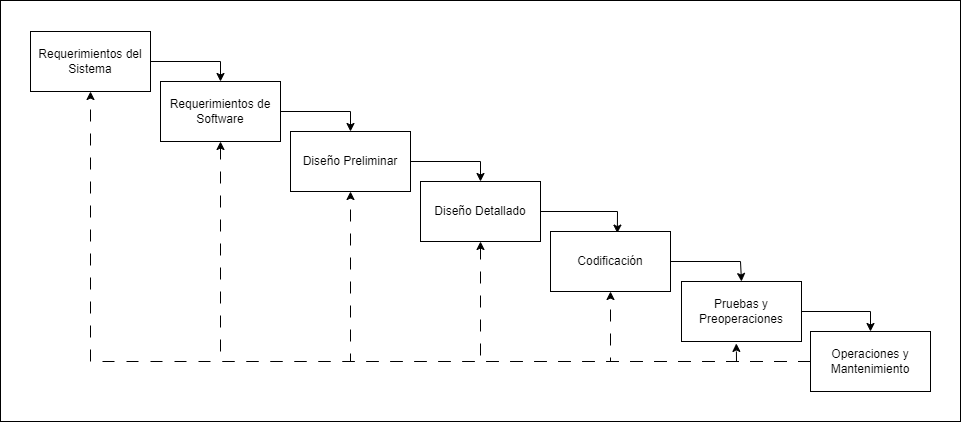
\includegraphics[width=1.0\textwidth]{images/marcoteorico/modelo_cascada.png}
	\caption{Proceso de desarrollo en Cascada.}
    \vspace{-0.2cm}
	\footnotesize{{Elaboración propia a partir de ``\textit{\citefield{auer1990solution}{title}}'' (\citeyear{auer1990solution}).}}
	\label{figs:modelo_desarrollo_cascada} 
\end{figure}
%--------------------------------------------------------------------------
\subsection{Agile}
Agile integra una filosofía y un conjunto de pautas para el desarrollo. Esta filosofía fomenta la satisfacción del cliente y la entrega incremental temprana del software mediante equipos de proyecto pequeños y altamente motivados, métodos informales y una simplificación general del proceso de desarrollo (\cite{pressman2005software}). Las pautas de desarrollo priorizan la entrega sobre el análisis y el diseño, manteniendo una comunicación activa y continua entre desarrolladores y clientes. En otras palabras, se centra en la entrega iterativa e incremental de software en lugar de seguir un enfoque lineal y secuencial. Entre algunas de los modelos de desarrollo bajo los principios de Programación ágil se distinguen: Scrum, Crystal, programación extrema, etc.\\ \indent
Más aun, entre las diversas metodologías ágiles existen herramientas de uso compartido. Por ejemplo, la revisión sistemática de literatura de \textcite{schon2017agile} identificó que los artefactos mas utilizados en la industria del software para obtener y entender los requerimientos del cliente son: Las \textbf{historias de usuario}, los \textbf{prototipos}, los diagramas de \textbf{casos de uso}, el análisis de \textbf{escenarios} y las \textbf{tarjetas de historia}.

\subsubsection{Programación Extrema}\hfill\\ 
\indent
Se trata de una metodología de desarrollo orientada a objetos cuyo objetivo es promover la aplicación de prácticas de ingeniería apropiadas para la creación de software. Como se puede notar en la Figura \ref{figs:modelo_desarrollo_xp}, bajo esta metodología, el proyecto se plantea en cuatro etapas: Planificación, diseño, programación y pruebas (\cite{pressman2005software}). 
\begin{figure}[H]
	\centering
	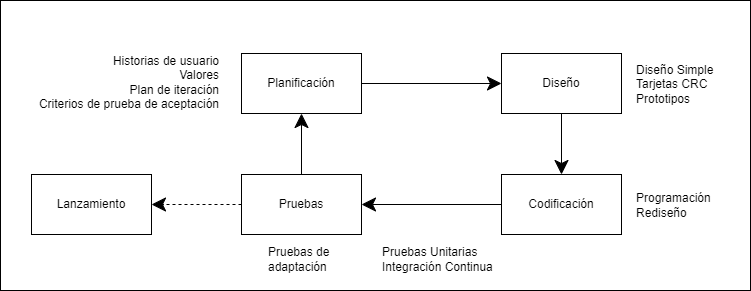
\includegraphics[width=1.0\textwidth]{images/marcoteorico/modelo_xp.png}
	\caption{Proceso de desarrollo bajo la metodología de Programación Extrema.}
    \vspace{-0.2cm}
	\footnotesize{{Elaboración propia a partir de ``\textit{\citefield{pressman2005software}{title}}'' (\citeyear{pressman2005software}).}}
	\label{figs:modelo_desarrollo_xp} 
\end{figure}
La planificación consta de escuchar a los clientes para comprender el contexto del negocio y definir las funcionalidades requeridas en forma de \textbf{historias} o \textbf{historias de usuario}. Cada historia es asignada un valor por el cliente basado en su importancia para el negocio, y el equipo de desarrollo estima el coste en semanas de desarrollo. Si una historia requiere más de tres semanas, se divide en historias más pequeñas. Luego, el equipo y el cliente deciden qué historias incluir en la próxima versión del software. Después de entregar la primera versión, se calcula la velocidad del proyecto, es decir, el número de historias implementadas. Este valor ayuda a estimar fechas de entrega y determinar si se ha comprometido demasiado en el proyecto. Durante el desarrollo, el cliente puede agregar, cambiar o eliminar historias, y el equipo ajusta sus planes en consecuencia.\\ \indent
El diseño sigue el principio de mantenerlo simple y se centra en proporcionar orientación de implementación para cada historia. Se utilizan tarjetas CRC (Clase Responsabilidad Colaborador) para identificar y organizar las clases relevantes en un contexto orientado a objetos. Se recomienda la creación de soluciones de prototipo operativas, llamadas soluciones de pico, para resolver problemas de diseño difíciles y validar estimaciones originales.\\ \indent
La programación se inicia después de desarrollar pruebas unitarias para cada historia. Se emplea la programación en pareja para mejorar la resolución de problemas en tiempo real y la calidad del código. Una vez completado el código, se integra continuamente con el trabajo de otros para evitar problemas de compatibilidad y se realiza pruebas de integración y validación a diario.
Finalmente, se desarrollan las pruebas de aceptación. Estas constan de la validación de las características y funcionalidades visibles y revisables por el cliente. 

\subsubsection{Scrum}\hfill\\ 
\indent
Scrum (nombre proveniente de una acción que tiene lugar durante un juego de rugby)  enfatiza el uso de un conjunto de patrones de proceso de software cuya efectividad ha sido probada. Cada uno de estos patrones a su vez define un conjunto de acciones a desarrollar. Estos patrones son:
\begin{itemize}[topsep=0pt]  
    \addtolength\itemsep{-4mm}
    \item \textbf{Backlog}: Una lista priorizada de requisitos o características del proyecto que proporcionan valor comercial para el cliente. Los elementos pueden agregarse al backlog en cualquier momento, lo que permite la introducción de cambios. El gerente de producto evalúa el backlog y actualiza las prioridades según sea necesario.
    \item \textbf{Sprints}: Consisten en unidades de trabajo necesarias para lograr un requisito definido en el backlog, que deben ajustarse a un plazo predefinido (generalmente 30 días o menos). Durante el sprint, no se introducen cambios (por ejemplo, elementos de trabajo del backlog), lo que permite que los miembros del equipo trabajen en un entorno a corto plazo pero estable.
    \item \textbf{Reuniones Scrum}: Reuniones cortas (generalmente de 15 minutos) celebradas diariamente por el equipo Scrum. Todos los miembros del equipo comparten información sobre lo que han hecho desde la última reunión, los obstáculos que están enfrentando y sus planes para la próxima reunión del equipo. Un líder de equipo, llamado Scrum master, lidera la reunión y evalúa las respuestas de cada persona. 
    \item \textbf{Demostraciones}: Entregan el incremento de software al cliente para que la funcionalidad implementada pueda ser demostrada y evaluada. Es importante tener en cuenta que la demostración puede no contener toda la funcionalidad planificada, sino solo aquellas funciones que pueden entregarse dentro del plazo establecido.
\end{itemize}
En síntesis, por medio de scrum, un equipo auto-organizado trabaja en entregas incrementales de funcionalidad (sprints), revisando y adaptando su trabajo en reuniones regulares (\cite{pressman2005software}). Esta dinámica queda ilustrada en la Figura \ref{figs:modelo_desarrollo_scrum}, la misma permite que un equipo de software trabaje con éxito en un mundo con requisitos cambiantes y críticos para el negocio.
\begin{figure}[H]
	\centering
	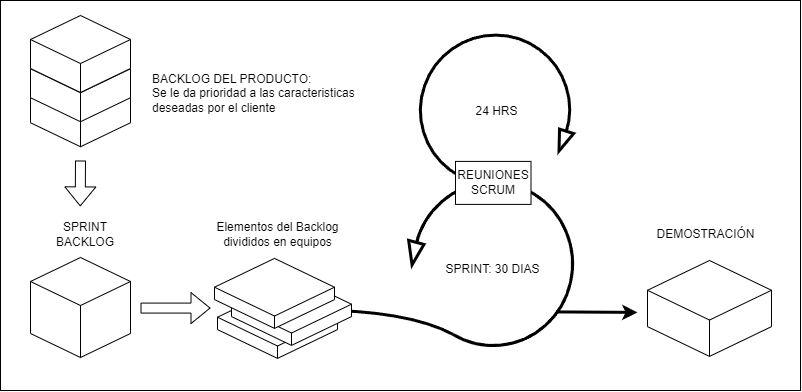
\includegraphics[width=1.0\textwidth]{images/marcoteorico/modelo_scrum.png}
	\caption{Proceso de desarrollo bajo la metodología Scrum.}
    \vspace{-0.2cm}
	\footnotesize{{Elaboración propia a partir de ``\textit{\citefield{pressman2005software}{title}}'' (\citeyear{pressman2005software}).}}
	\label{figs:modelo_desarrollo_scrum} 
\end{figure}

\subsubsection{Kanban}\hfill\\ 
\indent
Kanban, con "K" mayúscula, es un método de cambio evolutivo que utiliza un sistema de extracción kanban, visualización y otras herramientas para catalizar la introducción de ideas \textit{Lean} en el desarrollo tecnológico y las operaciones de tecnologías de la información (\cite{anderson2010kanban}). Kanban te permite lograr una optimización del proceso específica del contexto con una resistencia mínima al cambio, al mismo tiempo que mantiene un ritmo sostenible para los trabajadores involucrados.\\ \indent
El método Kanban se constituye de seis practicas que aportan un enfoque integral para la gestión de procesos en el desarrollo tecnológico y las operaciones.  La \textbf{visualización}, la \textbf{limitación del trabajo en proceso} y la \textbf{gestión del flujo} son pilares esenciales para comprender y controlar el trabajo en curso. Además, hacer explícitas las \textbf{políticas del proceso} y \textbf{implementar bucles de retroalimentación} permiten tomar decisiones basadas en datos objetivos y mejorar continuamente. Por último, el enfoque en \textbf{mejorar colaborativamente y evolucionar experimentalmente} impulsa al equipo hacia mejoras significativas y sostenibles en el tiempo (\cite{anderson2010kanban}).\\ \indent
Esto se logra mediante el uso de una pizarra o un tablero dividido en columnas y filas. Las columnas contienen las distintas tareas a realizar, mientras que las filas representan las prioridades de cada tarea. Las tareas se representan con tarjetas visuales que se mueven a lo largo de las columnas hasta completarse. Las columnas suelen tener los nombres \textbf{Tareas a iniciar o por hacer}, \textbf{Tareas en progreso} y \textbf{Tareas completadas}. Las filas se organizan en \textbf{Prioridad urgente}, \textbf{Prioridad importante} y \textbf{Prioridad no importante}(\cite{amaru2022sistema}).

%---------------------------------------------------------------------------------------------
%---------------------------------------------------------------------------------------------
\section{Análisis y Evaluación de Software}
En el análisis y evaluación de software, es fundamental considerar diversos modelos y estándares de calidad que guíen el desarrollo de productos de software, entre algunos de estos se encuentran los siguientes: 
%--------------------------------------------------------------------------
\subsection{Estándar ISO 25000:2014}
La ISO 25000, también conocida como SQuaRE (Requisitos y Evaluación de Calidad de Sistemas y Software), representa un conjunto de estándares diseñados para evaluar la calidad del software. Esta familia de normas facilita la organización, mejora y unificación de dos procesos fundamentales: la especificación de los requisitos de calidad del software y la evaluación de su calidad, respaldados por un proceso de medición específico. Surgiendo como una evolución de normativas previas como la ISO 9126, que detalla un modelo de calidad para productos de software, y la ISO 14598, centrada en la evaluación de estos productos, la norma ISO 25000 proporciona criterios para la especificación de requisitos de calidad, métricas y evaluación, así como un modelo de calidad que armoniza las definiciones de calidad de los clientes con los atributos durante el proceso de desarrollo (\cite{iso25000}).\\ \indent
La regulación consiste en cinco áreas principales, que abarcan desde la gestión hasta la evaluación de la calidad del producto software, dentro de la familia de normativas ISO 25000, estas son:

\begin{itemize}[topsep=0pt]  
    \addtolength\itemsep{-4mm}
    \item \textbf{ISO 2500n-Gestión de Calidad:} Este apartado define los modelos, términos y definiciones comunes que se utilizan en las otras normativas de la familia 25000.
    \item \textbf{ISO 2501n-Modelo de Calidad:} Se presentan modelos de calidad detallados incluyendo características para calidad interna, externa y en uso del producto software.
    \item \textbf{ISO 2502n-Medición de Calidad:}  Contiene modelos de referencia de la medición de la calidad del producto, definiciones de medidas de calidad tanto interna como externa y en uso además
    de guías practicas para su aplicación.
    \item \textbf{ISO 2503n-Requisitos de Calidad:} Especifica requisitos de calidad que pueden ser utilizados en el proceso de traslado de información de requisitos de calidad del producto software a desarrollar o como entrada del proceso de evaluación.
    \item \textbf{ISO 2504n-Evaluación de Calidad:} Proporciona requisitos, recomendaciones y guías para llevar a cabo el proceso de evaluación del producto software.
\end{itemize}

En consecuencia, con el propósito de asegurar que los atributos funcionales (como la adecuación, precisión, conformidad, interoperatividad y seguridad) y los no funcionales (como la fiabilidad, usabilidad, eficiencia, mantenibilidad y portabilidad) sean cumplidos al máximo, se llevan a cabo diversas pruebas, tales como pruebas unitarias, de integración, de regresión, de sistemas, de desempeño, de carga, de estrés, entre otras.
%--------------------------------------------------------------------------
\subsection{Estándar ISO 12207:2017}
La norma ISO 12207:2017 establece un marco común para los procesos del ciclo de vida del software, proporcionando una terminología precisa que la industria del software puede emplear de manera consistente. Este estándar es aplicable tanto a programas nuevos como a los ya existentes, abarcando firmware, software independiente y software embebido. Define procesos, actividades y tareas aplicables a lo largo de la adquisición, suministro, desarrollo, operación, mantenimiento y desecho de sistemas, productos y servicios informáticos, con el propósito de satisfacer las necesidades del cliente (\cite{amaru2022sistema}).\\
La norma clasifica los procesos en tres categorías principales: primarios, de soporte y organizacionales. Los procesos primarios abarcan la adquisición, suministro, desarrollo, operación y mantenimiento del software. Los procesos de soporte incluyen la documentación, gestión de configuración, aseguramiento de calidad, verificación, validación, revisión conjunta, auditoría y resolución de problemas. Por último, los procesos organizacionales comprenden la gestión, mejora, infraestructura y gestión de recursos humanos.\\
Dentro de un proyecto, es crucial identificar uno o más modelos de desarrollo, como cascada, incremental, evolutivo, reingenieria o espiral, entre otros. Las características del proyecto deben definir los requisitos y especificaciones del producto o servicio, los cuales guían la determinación y selección de procesos, actividades y tareas a emplear.
%--------------------------------------------------------------------------
\subsection{Estándar ISO 420001:2023}
La norma ISO 42001 es un estándar internacional que detalla los requisitos para establecer, implementar, mantener y mejorar de manera continua un Sistema de Gestión de Inteligencia Artificial (SGIA) en las organizaciones. Su propósito es asegurar un desarrollo y uso responsables de los sistemas de IA, tanto para entidades que proveen como para aquellas que utilizan productos o servicios basados en esta tecnología. Esta norma aborda los desafíos únicos que presenta la IA, incluyendo consideraciones éticas, transparencia y aprendizaje continuo. Proporciona a las organizaciones una estructura sólida para gestionar los riesgos y las oportunidades asociadas con la IA, al mismo tiempo que equilibra la innovación con la gobernanza (ISO \citeyear{iso42001}).\\
Esta normativa está basada en la ISO 22989; Esta normativa describe los conceptos, definiciones, ciclo de vida y aplicaciones de la inteligencia artificial. Este documento define un sistema de inteligencia artificial como un sistema diseñado que genera salidas tales como contenido, pronósticos, recomendaciones o decisiones para un conjunto dado de objetivos definidos por humanos. Los sistemas de IA no entienden; necesitan elecciones de diseño humano, ingeniería y supervisión. El grado de supervisión depende del caso de uso, pero como mínimo, la supervisión está presente durante el entrenamiento y la validación (ISO \citeyear{iso22989}).
Las directrices establecidas en estas norma son de naturaleza genérica y pueden aplicarse a cualquier tipo de organización, independientemente de su forma jurídica, tamaño o ámbito de actividad. Esto implica que es igualmente aplicable tanto a entidades públicas como privadas.

%---------------------------------------------------------------------------------------------
%---------------------------------------------------------------------------------------------
% 10 paginas
\section{Inteligencia Artificial}
La IA es una rama de la ciencia de la computación que se dedica a abordar desafíos cognitivos, principalmente asociados a la inteligencia humana, tales como el proceso de aprendizaje, la resolución de problemas y la identificación de patrones (\cite{kim2019implementation}). Por tanto, el desarrollo de sistemas de inteligencia artificial tienen como finalidad la construcción de sistemas informáticos que puedan ejecutar actividades que comúnmente implican inteligencia humana. Mientras que la programación tradicional depende de los programadores para definir lógica e instrucciones explícitas específicas de escenarios, ML permite a las máquinas aprender de manera autónoma y tomar decisiones sin instrucciones detalladas para cada tarea. Naturalmente estos sistemas, dotados de inteligencia artificial, se diseñan para reconocer ciertos contextos y tomar decisiones para satisfacer ciertas necesidades (\cite{iso22989}).  Más aun, es importante considerar que los sistemas de IA no se basan en una única tecnología, sino en una combinación de varias como se ilustra en la Figura \ref{figs:ai_ecosystem}.
\begin{figure}[htb]
	\centering
	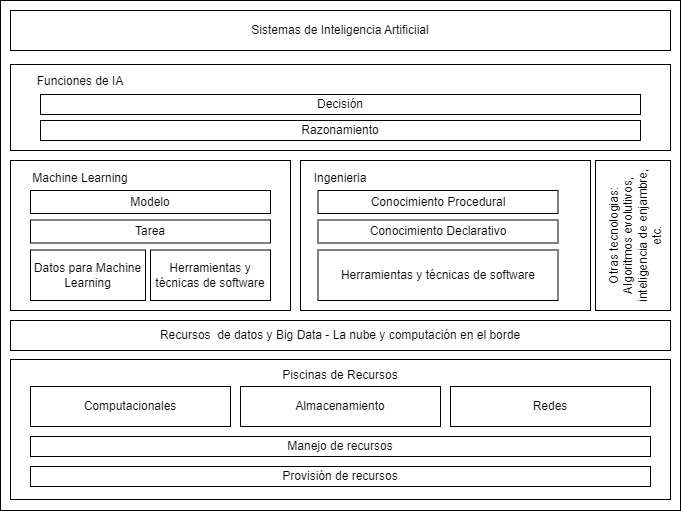
\includegraphics[width=1.0\textwidth]{images/marcoteorico/ai_ecosystem.png}
	\caption{Ecosistema de un sistema de inteligencia artificial.}
    \vspace{-0.2cm}
	\footnotesize{{Elaboración propia a partir de ``\textit{\citefield{iso22989}{title}}'' (\citeyear{iso22989}).}}
	\label{figs:ai_ecosystem} 
\end{figure}

%---------------------------------------------------------------------------------------------
\subsection{Aprendizaje}
En función de si requieren o no de grandes cantidades de datos para aprender, los sistemas de IA se puede categorizar en dos grandes categorías: Basados en heurística y basados en aprendizaje automático. 

\subsubsection{Sistemas basados en heuristica}\hfill\\ 
\indent
Los sistemas de IA que no implican aprendizaje se llaman heurísticos. Los sistemas expertos clásicos o sistemas de razonamiento equipados con una base de conocimientos fija son algunos ejemplos de este tipo de sistemas. En estos casos, los desarrolladores del sistema aprovechan el conocimiento humano para proporcionar reglas razonables para el comportamiento del sistema de IA.\\ 
\indent
Es importante diferenciar una heurística de un algoritmo, la heurística es una suposición que sirve como guía inicial para exploraciones posteriores. A diferencia de un algoritmo, los resultados de una heurística no son predecibles ni reproducibles. Más aun, cuando un algoritmo utiliza una heurística, ya no necesita analizar exhaustivamente todas las posibles soluciones, por lo que puede encontrar soluciones aproximadas más rápidamente a costa de precisión y exhaustividad.

\subsubsection{Sistemas basados en aprendizaje automatico}\hfill\\ 
\indent
Los sistemas de IA que implican aprendizaje se denominan sistemas basados en aprendizaje automático. El aprendizaje implica análisis computacionales de un conjunto de datos de entrenamiento para detectar patrones, construir un modelo y comparar la salida del modelo resultante con los comportamientos esperados;Este proceso se conoce como entrenamiento. La base de conocimientos resultante es un modelo entrenado basado en una función matemática y un conjunto de entrenamiento que representa la mejor aproximación del comportamiento basada en un entorno dado.

\begin{comment}

%---------------------------------------------------------------------------------------------
\subsection{Redes Neuronales}
\subsubsection{Estructura de una Red Neuronal}
\subsubsection{Tipos de Redes Neuronales Artificiales}

%---------------------------------------------------------------------------------------------
\subsection{Visión Computacional}
\subsubsection{Reconocimiento Óptico de Caracteres (OCR)}\hfill\\ 
\indent
(\cite{huggingface2022documentai}).

%---------------------------------------------------------------------------------------------
\subsection{Procesamiento de Lenguaje Natural(PLN)}

\subsubsection{Arquitectura de un Sistema PLN}
\subsubsection{Minería de Texto}
\subsubsection{Analisis de Texto y Categorización}
\subsubsection{Procesamiento Lingüistico}
\subsubsection{Analisis de Subjetividad}

%---------------------------------------------------------------------------------------------
\subsection{Generación de Lenguaje Natural(GLN)}
\subsubsection{GLN basado en plantillas}
\subsubsection{GLN a partir de imagenes}

%---------------------------------------------------------------------------------------------
%---------------------------------------------------------------------------------------------
% 1 pagina 
\section{Trabajos Relacionados}
\end{comment}